% Apresentação de Qualificação de Mestrado
% AIPE: Seleção Contextual de Políticas de Reposição em Redes Varejistas
% Compilar com: latexmk -xelatex main.tex  (ver Makefile)
\documentclass[11pt,aspectratio=169]{beamer}

\usetheme{metropolis}

% --- Idioma e fontes ---
\usepackage{fontspec}
\usepackage{polyglossia}
\setdefaultlanguage[variant=brazilian]{portuguese}

% --- Pacotes de suporte ---
\usepackage{booktabs}
\usepackage{makecell}
\usepackage{colortbl}
\usepackage{graphicx}
\usepackage{tikz}
\usetikzlibrary{positioning,arrows.meta,fit,backgrounds,calc}
\usepackage{amsmath}
\usepackage{textcomp}

% --- Paleta sóbria: azul escuro, cinza, branco, destaque discreto ---
\definecolor{darkblue}{HTML}{1B3A5C}
\definecolor{slategray}{HTML}{5B6B79}
\definecolor{lightgray}{HTML}{EDEFF1}
\definecolor{accenteal}{HTML}{3E7C8C}
\definecolor{warnred}{HTML}{8C3E3E}

\setbeamercolor{palette primary}{bg=darkblue,fg=white}
\setbeamercolor{palette secondary}{bg=slategray,fg=white}
\setbeamercolor{palette tertiary}{bg=darkblue,fg=white}
\setbeamercolor{frametitle}{bg=darkblue,fg=white}
\setbeamercolor{progress bar}{fg=accenteal,bg=lightgray}
\setbeamercolor{alerted text}{fg=accenteal}
\setbeamercolor{normal text}{fg=black!85}

\setbeamertemplate{frame numbering}[fraction]
\metroset{block=fill,sectionpage=progressbar,numbering=fraction,progressbar=frametitle}

% --- Comandos auxiliares de estilo ---
\newcommand{\highlight}[1]{\textcolor{accenteal}{\textbf{#1}}}
\newcommand{\fonte}[1]{{\footnotesize\textcolor{slategray}{Fonte: #1}}}

\title{Seleção Contextual de Políticas de Reposição em Redes Varejistas}
\subtitle{O AIPE como \textit{framework} metodológico de apoio à decisão}
\author{Matheus Inácio Batista Santos}
\institute{\small Instituto de Computação --- UFAL\\
\scriptsize Orientadores: Dr. Rian G. S. Pinheiro e Dr. Bruno C. S. Nogueira}
\date{\small Exame de Qualificação de Mestrado}

\begin{document}

\input{sections/s01_titulo}
\input{sections/s02_problema_em_uma_frase}
% Slide 3 — Heterogeneidade da demanda
\begin{frame}{Heterogeneidade da demanda}
  \begin{columns}[T,onlytextwidth]
    \column{0.46\textwidth}
      \textbf{Produto regular}\\
      \small Vende com previsibilidade (ex.: 50 un./semana em qualquer loja).
      \vspace{0.8em}

      \textbf{Produto intermitente / \textit{lumpy}}\\
      \small Períodos de demanda nula intercalados com picos esporádicos
      (ex.: ``0, 0, 0, 50, 0, 0, 30'').
    \column{0.5\textwidth}
      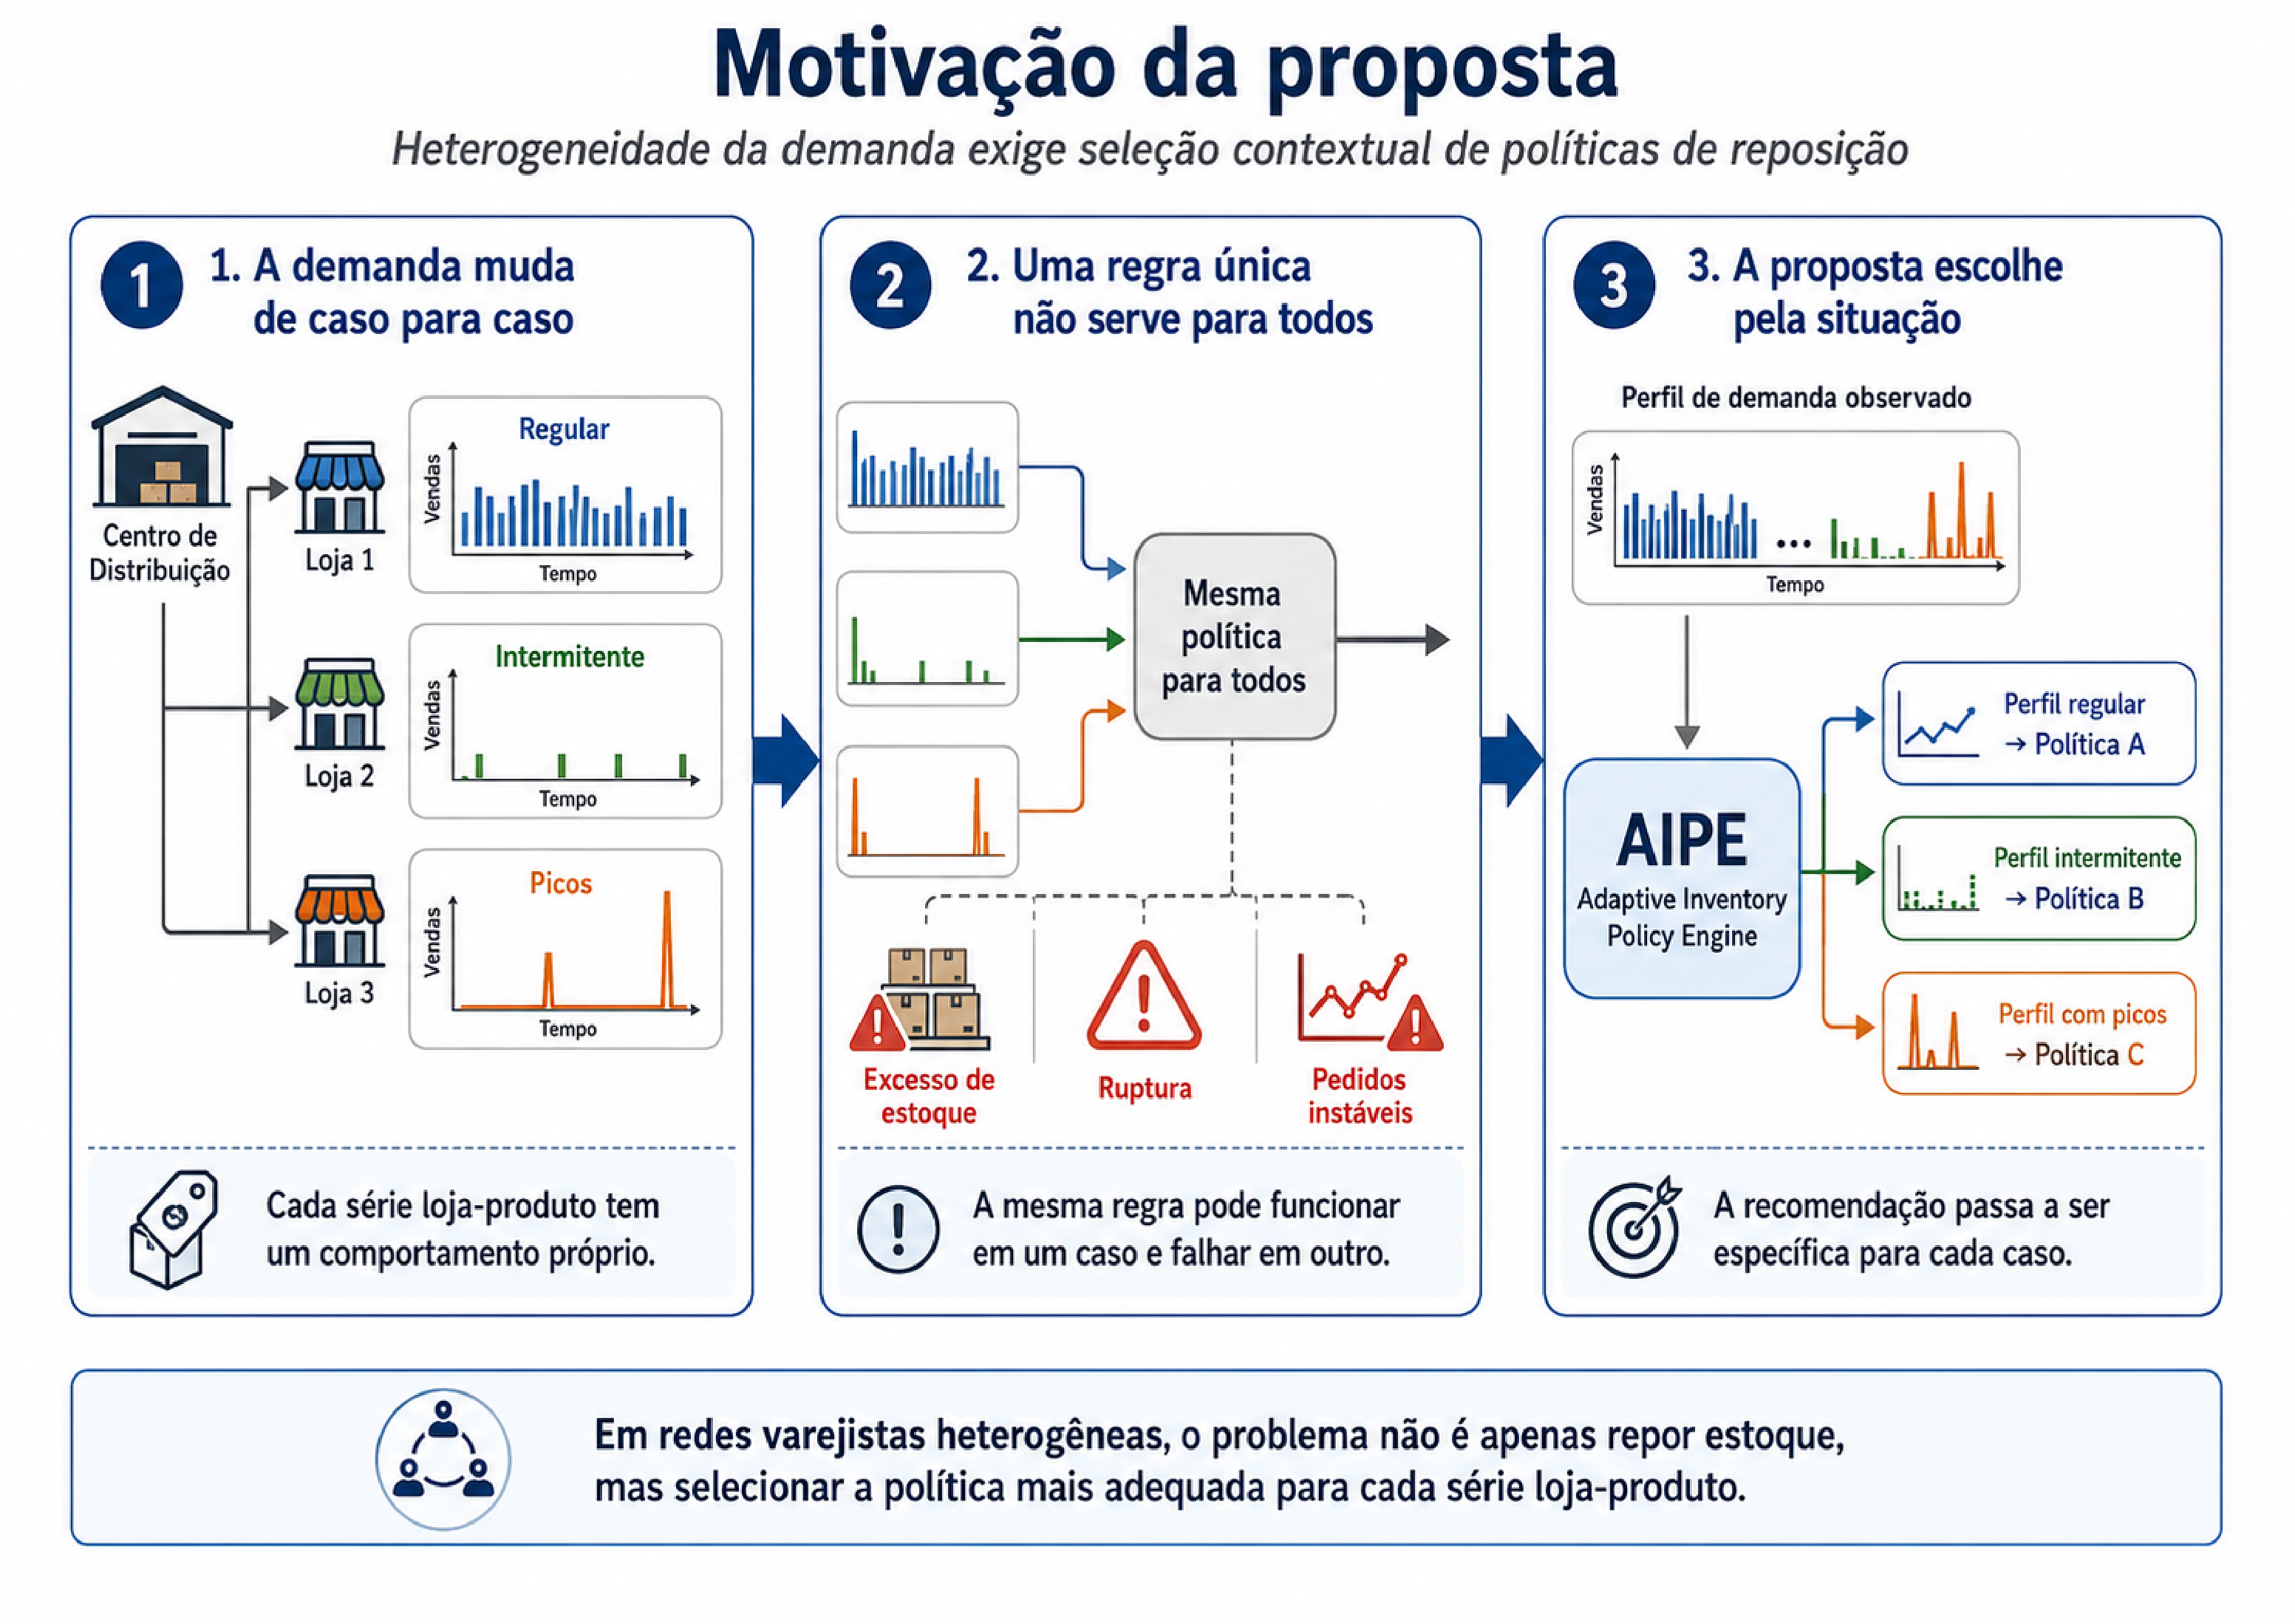
\includegraphics[width=\linewidth,height=4.6cm,keepaspectratio]{figures/figura_1_1_motivacao_aipe.pdf}
  \end{columns}
  \vfill
  \begin{alertblock}{Mesma rede, padrões distintos}
    \small Aplicar a \highlight{mesma política} a séries com comportamentos tão
    diferentes tende a ser ineficiente.
  \end{alertblock}
  \note{
    O ponto central aqui é visual: dentro da mesma rede varejista, produtos
    diferentes (ou o mesmo produto em lojas diferentes) podem ter padrões de
    venda completamente distintos. Uns vendem de forma regular e previsível;
    outros têm longos períodos sem nenhuma venda, seguidos de picos grandes
    e irregulares — isso é o que a literatura chama de demanda intermitente
    ou \textit{lumpy}. Essa figura, que está no Capítulo 1 da dissertação,
    ilustra exatamente essa heterogeneidade que motiva todo o trabalho.
  }
\end{frame}

\input{sections/s04_consequencias_operacionais}
\input{sections/s05_pergunta_pesquisa}
\input{sections/s06_hipotese}
% Slide 7 — Lacuna na literatura
\begin{frame}{A lacuna não é falta de algoritmos}
  \begin{columns}[T,onlytextwidth]
    \column{0.55\textwidth}
      \textbf{O que já existe}
      \begin{itemize}
        \small
        \item Modelos analíticos clássicos (EOQ, $(s,S)$, Jornaleiro)
        \item Políticas parametrizadas por meta-heurísticas
        \item Políticas aprendidas por reforço
        \item Comparações isoladas entre famílias
      \end{itemize}
    \column{0.45\textwidth}
      \textbf{O que falta}
      \begin{itemize}
        \small
        \item \highlight{Seleção contextual} validada em dados reais
        \item Evidência em \highlight{varejo brasileiro} intermitente
        \item Ligação explícita entre perfil e política dominante
      \end{itemize}
  \end{columns}
  \vfill
  \begin{alertblock}{Posicionamento}
    \small O problema se aproxima da \textbf{seleção de algoritmos}
    (Rice, 1976) -- escolher, para cada instância, a alternativa com melhor
    desempenho esperado.
  \end{alertblock}
  \note{
    A literatura de controle de inventário já oferece muitas alternativas:
    modelos analíticos, meta-heurísticas, aprendizado por reforço. O que
    falta não é mais um algoritmo -- é um mecanismo de seleção contextual
    validado sobre dados reais, especialmente em um contexto pouco coberto,
    que é o varejo brasileiro com demanda intermitente. A formulação que eu
    adoto se aproxima do problema clássico de seleção de algoritmos, de
    Rice, 1976: dado um conjunto de instâncias e um portfólio de
    alternativas, aprender a escolher a alternativa mais adequada para
    cada instância.
  }
\end{frame}

\input{sections/s08_contribuicao}
\input{sections/s09_visao_geral_aipe}
\input{sections/s10_entradas_aipe}
\input{sections/s11_caracterizacao_pods}
\input{sections/s12_ambiente_simulacao_metricas}
\input{sections/s13_portfolio_politicas}
\input{sections/s14_rotulos_pse}
\input{sections/s15_experimento1_pb}
% Slide 16 — Experimento 2: Bahia
\begin{frame}{Experimento 2: expansão na Bahia}
  \begin{columns}[T,onlytextwidth]
    \column{0.42\textwidth}
      \textbf{Escopo}
      \small
      \begin{itemize}
        \item 145 séries (loja, produto)
        \item 3 filiais, 6 segmentos comerciais
        \item 12 políticas $\times$ 5 replicações
        \item 8.700 pontos de avaliação
        \item Regime \textit{Lumpy} (71\% das séries)
      \end{itemize}
    \column{0.58\textwidth}
      \centering
      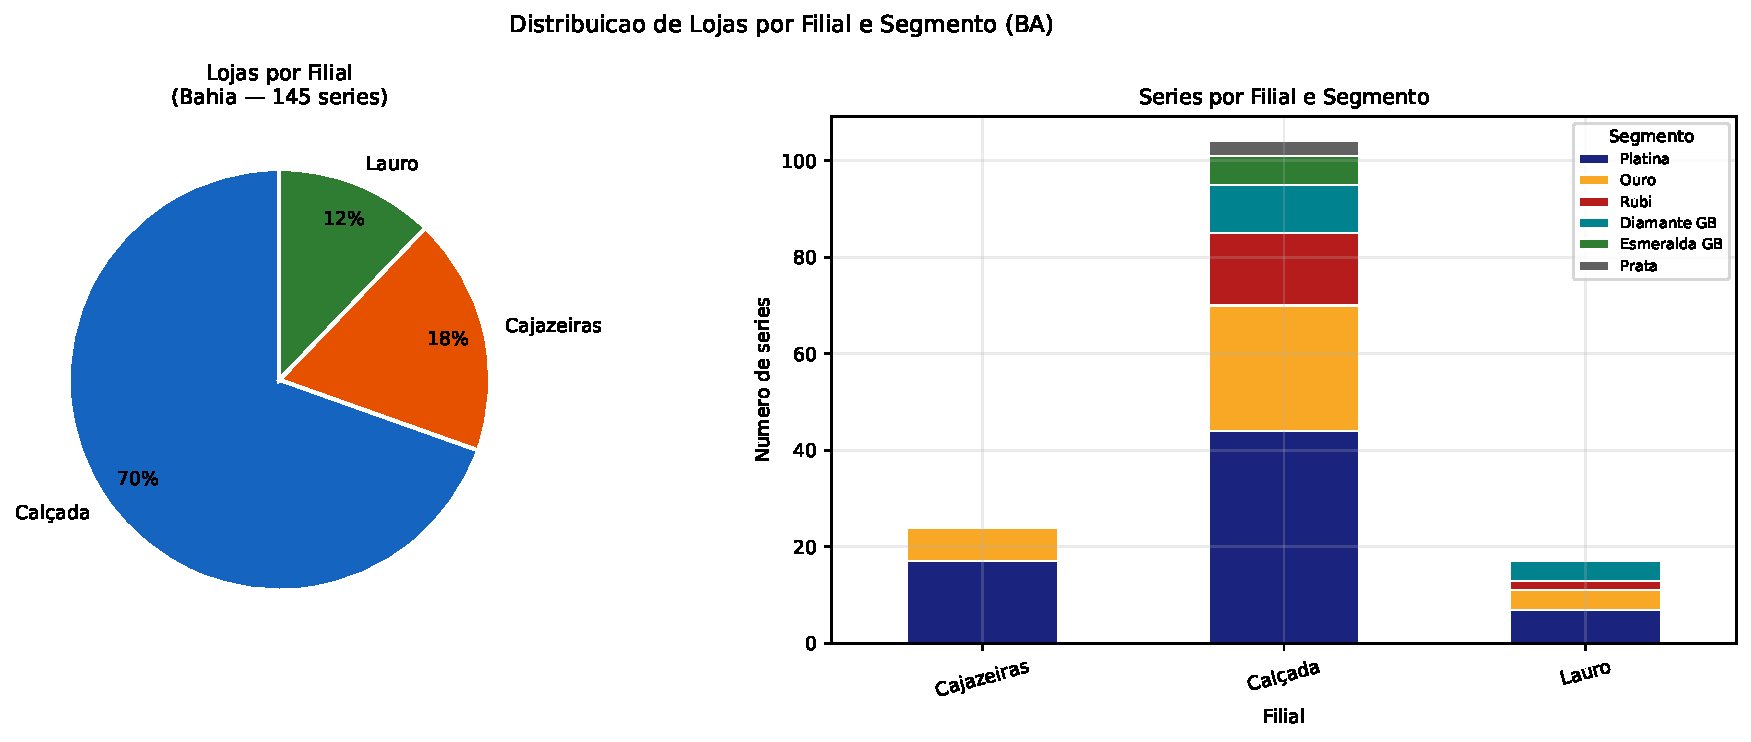
\includegraphics[width=\linewidth]{figures/distribuicao_lojas_segmento.pdf}
  \end{columns}
  \vspace{0.3em}
  \small \fonte{simulation/data/08\_reporting/maps/distribuicao\_lojas\_segmento}
  \note{
    O Experimento 2 amplia a escala: 145 combinações loja-produto do estado
    da Bahia, com cinco replicações independentes por política, totalizando
    8.700 pontos de avaliação. Isso habilita testes estatísticos formais,
    algo que o piloto da Paraíba não permitia com apenas uma replicação.
    A figura mostra como essas séries se distribuem entre as três filiais
    e os seis segmentos comerciais da rede -- a filial Calçada concentra
    72% das séries, o que é importante para interpretar os resultados
    agregados que vêm a seguir.
  }
\end{frame}

% Slide 17 — Nenhuma política domina simultaneamente
\begin{frame}{Nenhuma política domina simultaneamente}
  \begin{columns}[T,onlytextwidth]
    \column{0.5\textwidth}
      \centering
      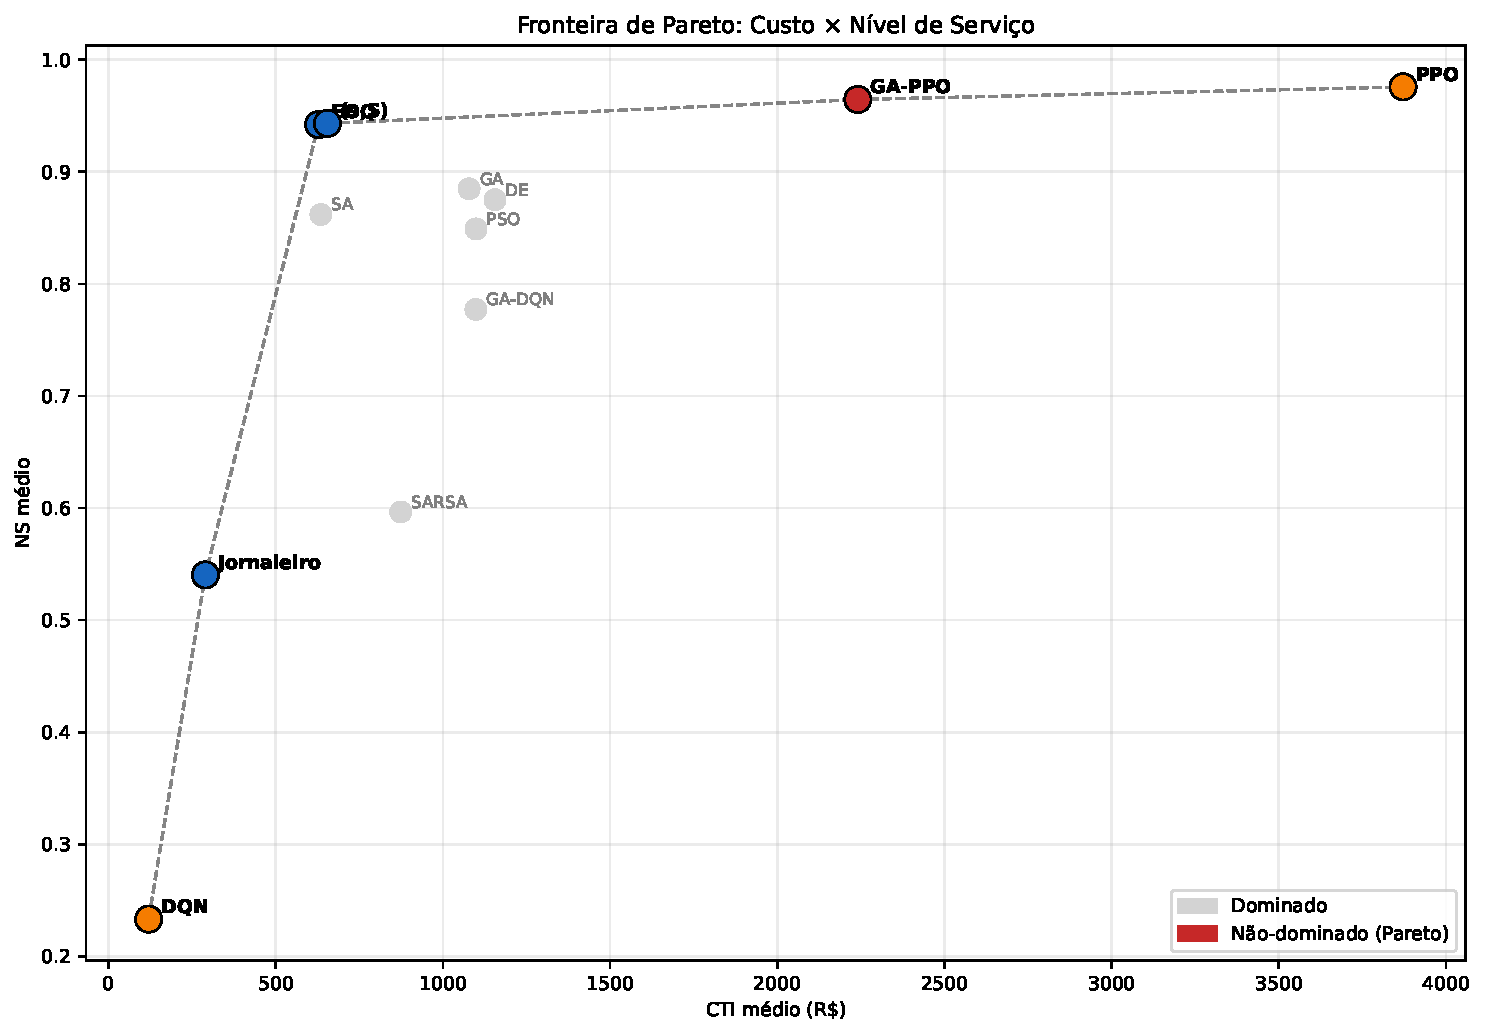
\includegraphics[width=\linewidth]{figures/pareto_frontier.pdf}\\
      \scriptsize Fronteira de Pareto CTI--NS
    \column{0.5\textwidth}
      \centering
      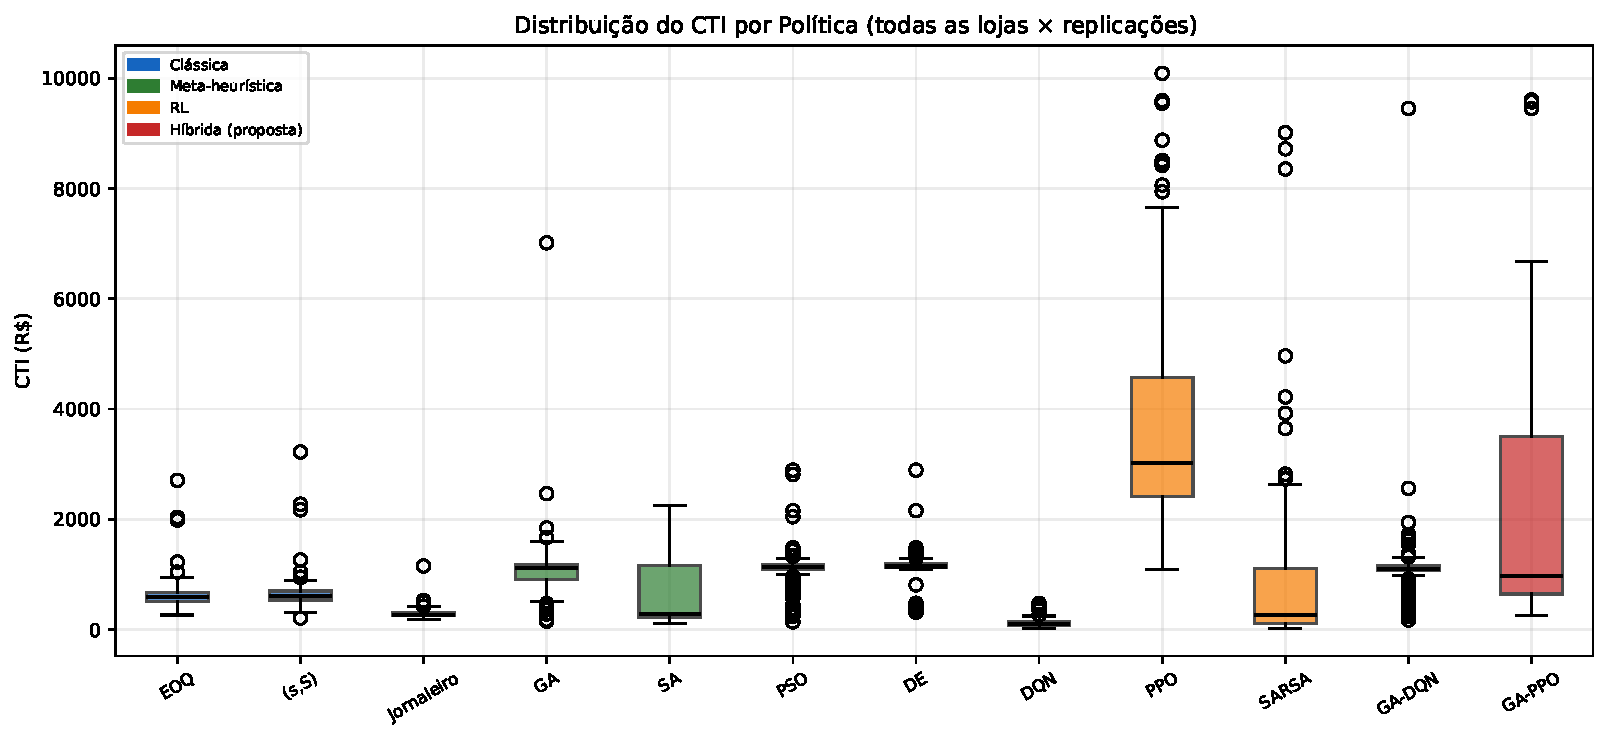
\includegraphics[width=\linewidth]{figures/boxplot_tic.pdf}\\
      \scriptsize Dispersão de CTI por política
  \end{columns}
  \vspace{0.5em}
  \small Sobre as 145 séries da Bahia: \highlight{EOQ} e $(s,S)$ oferecem o
  melhor equilíbrio custo-serviço agregado (NS\,$=$\,0,94); o
  \highlight{Jornaleiro} tem o menor custo bruto, mas NS\,$=$\,0,54.
  \note{
    Estas duas figuras resumem a evidência empírica central do Experimento
    2. À esquerda, a fronteira de Pareto entre CTI e NS mostra que nenhum
    ponto ocupa simultaneamente o menor custo e o maior nível de serviço --
    quem prioriza custo aponta para o Jornaleiro, quem prioriza serviço
    aponta para EOQ ou (s,S). À direita, o boxplot mostra que a mesma
    política produz custos muito diferentes entre séries -- a eficácia
    depende do perfil da demanda, não só da política escolhida. Essa
    heterogeneidade é a evidência empírica direta que justifica a
    necessidade de seleção contextual.
  }
\end{frame}

\input{sections/s18_politica_unica_vs_perfil}
% Slide 19 — Evidência de heterogeneidade por perfil
\begin{frame}{Dominância depende do perfil operacional}
  \begin{columns}[T,onlytextwidth]
    \column{0.52\textwidth}
      \centering
      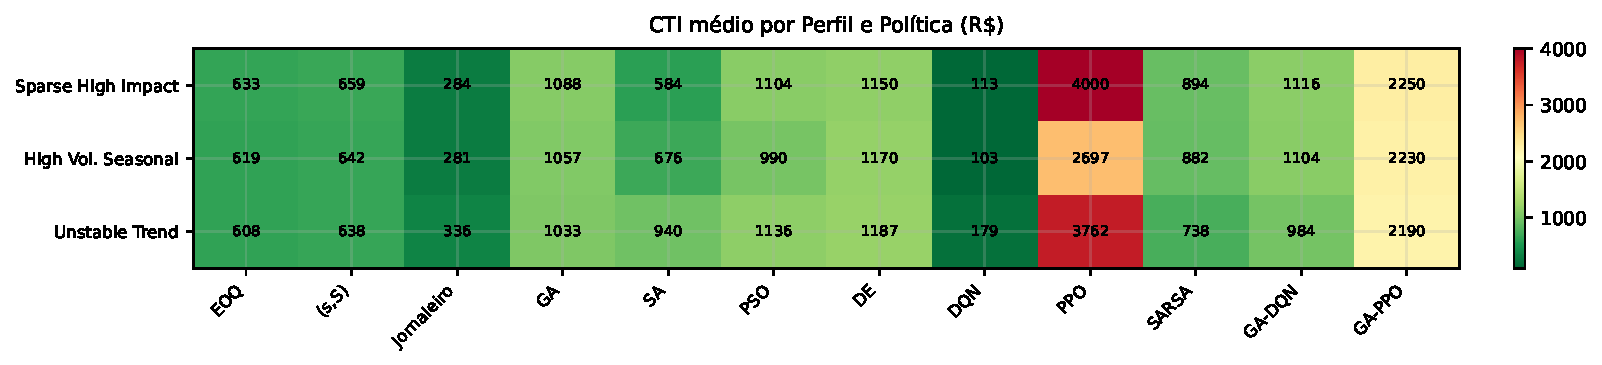
\includegraphics[width=\linewidth]{figures/profile_policy_heatmap_cti.pdf}\\
      \scriptsize CTI médio por política e POD
    \column{0.48\textwidth}
      \centering
      \resizebox{\linewidth}{!}{%
      \begin{tabular}{@{}lcrr@{}}
        \toprule
        \textbf{Perfil} & $n$ & \textbf{Dominante} & \textbf{CTI (R\$)} \\
        \midrule
        Sparse High Impact & 116 & SA & 584,01 \\
        Unstable Trend & 18* & EOQ & 607,95 \\
        High Vol. Seasonal & 11* & EOQ & 618,79 \\
        \bottomrule
      \end{tabular}}\\[0.4em]
      \scriptsize *$n<20$: evidência exploratória.
  \end{columns}
  \vspace{0.6em}
  \begin{alertblock}{Cuidado com o custo bruto}
    \small O Jornaleiro tem o \highlight{menor CTI bruto} em Sparse High
    Impact (R\$\,284), mas NS\,$=$\,0,55 -- abaixo do limiar de viabilidade
    de 0,70. Não é dominante: o ganho de custo não é alcançável sem violar
    o nível de serviço mínimo.
  \end{alertblock}
  \note{
    O heatmap mostra como o custo médio de cada política varia conforme o
    perfil operacional -- nenhuma célula é a mais clara em todas as linhas
    e colunas simultaneamente, o que é a evidência visual direta da
    heterogeneidade. A tabela à direita resume a política dominante por
    perfil, sempre sob a restrição de NS mínimo de 0,70: SA domina no
    perfil que concentra 80% das séries; EOQ domina nos dois perfis
    menores, que têm evidência exploratória por terem menos de 20 séries.
    É essencial destacar a ressalva do Jornaleiro: ele tem o menor custo
    bruto no perfil mais numeroso, mas seu nível de serviço de 0,55 está
    muito abaixo do limiar mínimo -- por isso ele é excluído da dominância,
    mesmo sendo o mais barato. Isso evita uma leitura simplista de que
    custo baixo implica política melhor.
  }
\end{frame}

% Slide 20 — CTI ajustado e estabilidade operacional
\begin{frame}{CTI ajustado por estabilidade (análise complementar)}
  \begin{columns}[T,onlytextwidth]
    \column{0.48\textwidth}
      \centering
      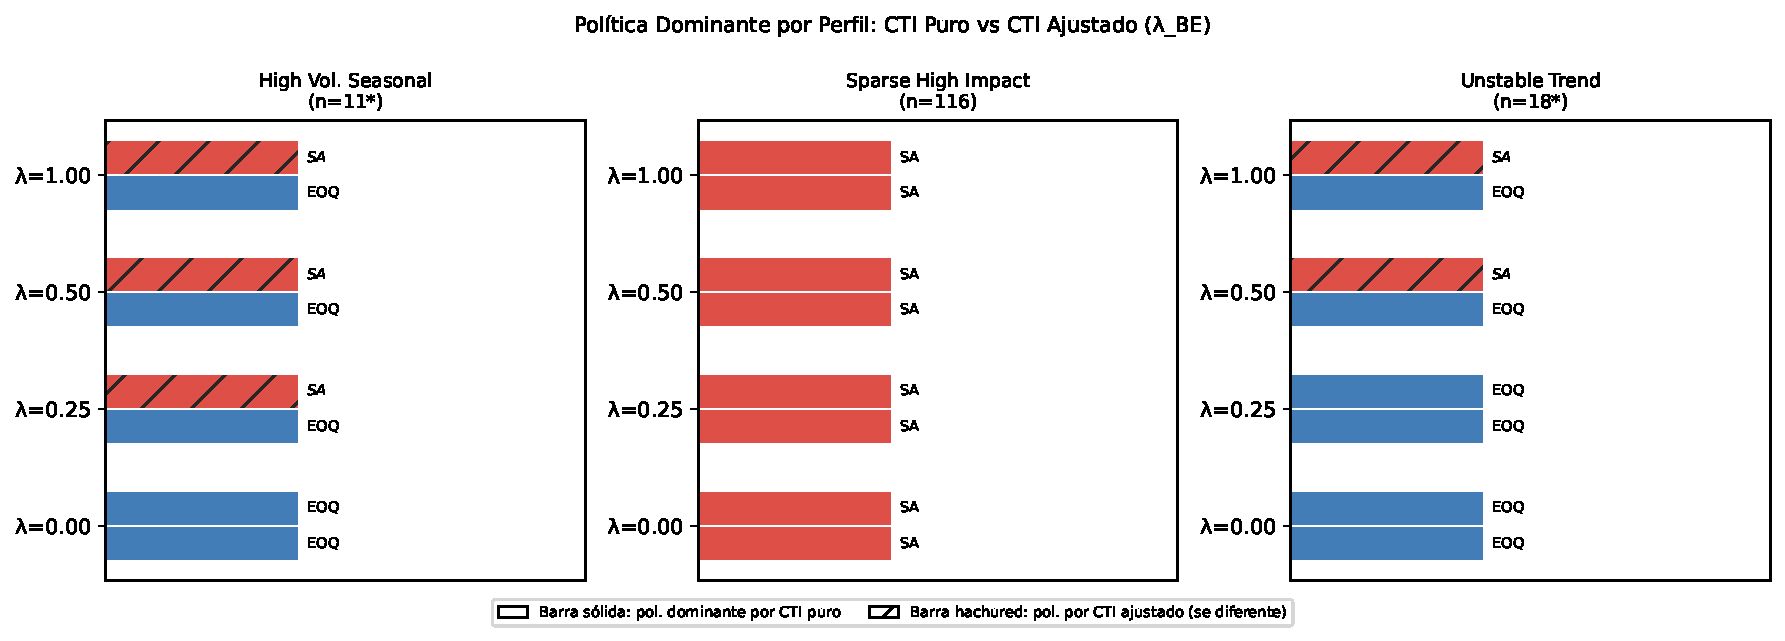
\includegraphics[width=\linewidth]{figures/cti_adjusted_sensitivity.pdf}\\
      \scriptsize Sensibilidade a $\lambda_{BE}$
    \column{0.52\textwidth}
      \small
      $J(\pi,g) = \mathrm{CTI}_{\text{norm}} + \lambda_{BE}\cdot \mathrm{BE}_{\text{norm}}$
      \vspace{0.5em}

      \begin{itemize}
        \small
        \item $\lambda_{BE}=0$: recupera o CTI puro (EOQ domina)
        \item $\lambda_{BE}\geq 0{,}25$: política única migra para
          \highlight{SA} (BE\,$=$\,5,5 vs.\ 55,4 do EOQ)
        \item Em $\lambda_{BE}=1{,}0$: até +56,6\% de redução ajustada,
          com NS caindo de 0,942 para 0,862
      \end{itemize}
  \end{columns}
  \vspace{0.4em}
  \begin{alertblock}{Status: preliminar e complementar}
    \footnotesize Não substitui o critério principal (CTI puro sob NS
    $\geq 0{,}70$). A partir de $\lambda_{BE}\geq 0{,}5$, a seleção por perfil
    converge para a política única ajustada.
  \end{alertblock}
  \note{
    Além do CTI puro, reportamos uma análise de sensibilidade que penaliza
    o custo normalizado pelo efeito bullwhip normalizado, com peso lambda.
    Com lambda zero, recuperamos exatamente o critério principal. Conforme
    lambda aumenta, a política única ótima migra do EOQ -- que tem BE muito
    alto, 55,4 -- para o SA, que é muito mais estável, com BE de 5,5,
    produzindo reduções de custo ajustado maiores, de até 56,6%, mas com
    queda adicional de nível de serviço. É fundamental destacar que essa é
    uma análise preliminar e complementar -- o critério principal da
    dissertação continua sendo o CTI puro sob a restrição de NS mínimo.
    Notem também que, quando a penalidade por instabilidade domina, a
    seleção por perfil perde sua vantagem diferenciadora, porque a política
    mais estável passa a ser preferida uniformemente em todos os perfis.
  }
\end{frame}

\input{sections/s21_limitacoes}
\input{sections/s22_plano_continuidade}
\input{sections/s23_fechamento}

\end{document}
